\chapter{驯化植物}\label{ch:g12:domesticated-plants}

在一穗现代玉米旁边——六百粒籽粒整齐排成行，
包裹在苞叶中，紧紧固定在穗轴上——旁边摆着
大刍草的穗，即玉米的野生祖先：仅一排十二粒籽粒，
每粒都包着坚硬的外壳，成熟时逐粒脱落。
九千年的挑选中，农民留下所偏爱植株的
种子，把前者变成了后者。
这一结果离开人类便无法存活一个季节：田间遗落的玉米穗
会就地腐烂。本章讨论的是，当人类成为植物的选择环境时，
植物会发生怎样的变化——以及人们有意改变植物\omterm{def:g10:universal-dna:gene}{基因}的
较新方法。

\section{人类的选择}

\begin{definition}[驯化、人工选择]\label{def:g12:domesticated-plants:domestication}
\emph{驯化}\index{驯化}是将一种野生\omterm{def:g10:biodiversity-scales:species}{物种}
转变为依赖人类、为人类服务的\omterm{def:g10:biodiversity-scales:species}{物种}，通过
\emph{人工选择}\index{人工选择}：每一代中，
人们保留并播种具有所需性状个体的种子，
使这些性状背后的\omterm{def:g10:universal-dna:gene}{等位基因}的频率上升。
它就是\cref{ch:g12:selection-drift-speciation}中的选择，
只是以人的眼光取代环境，其作用机制相同——
但速度更快，因为选择是有意且严厉的。
\end{definition}

\begin{proposition}[驯化选择的性状]\label{prop:g12:domesticated-plants:traits}
作物共有一组野生植物不会保留的性状，即
\emph{\omterm{def:g12:domesticated-plants:domestication}{驯化}综合征}：种子留在植株上而不散落（不落粒的穗）；
种子和果实更大；
种子立即萌发，而非在土壤中等待数年；
毒素与苦味防御物质的丧失；植株紧凑，
分枝少，只结一个大穗而非多个小穗；以及
成熟同步。每一项对收获者有利，
而对植株本身却有害——作物是为了人类的便利、
违背其独立性而被选出的植株。
\end{proposition}
\begin{proof}[证据]
野生小麦从易断的穗轴上落粒；最早的栽培小麦
见于最古老的农耕遗址，其穗轴坚韧，能够保住籽粒——
收割者的镰刀无意中选中了籽粒留在植株上的\omterm{def:g11:mutations:mutation}{突变}体，
便于人们收集并播种。
大刍草与玉米仅在约五个主要\omterm{def:g10:universal-dna:gene}{基因}上存在差异：其中一个
使多分枝的植株变为单一茎秆，另一个使籽粒脱出硬壳，
其余\omterm{def:g10:universal-dna:gene}{基因}则增加了行数。二者杂交
可得可育后代，中间类型也确实存在：同一\omterm{def:g10:biodiversity-scales:species}{物种}，
只是形态被重新塑造。
\end{proof}

\begin{omfigure}
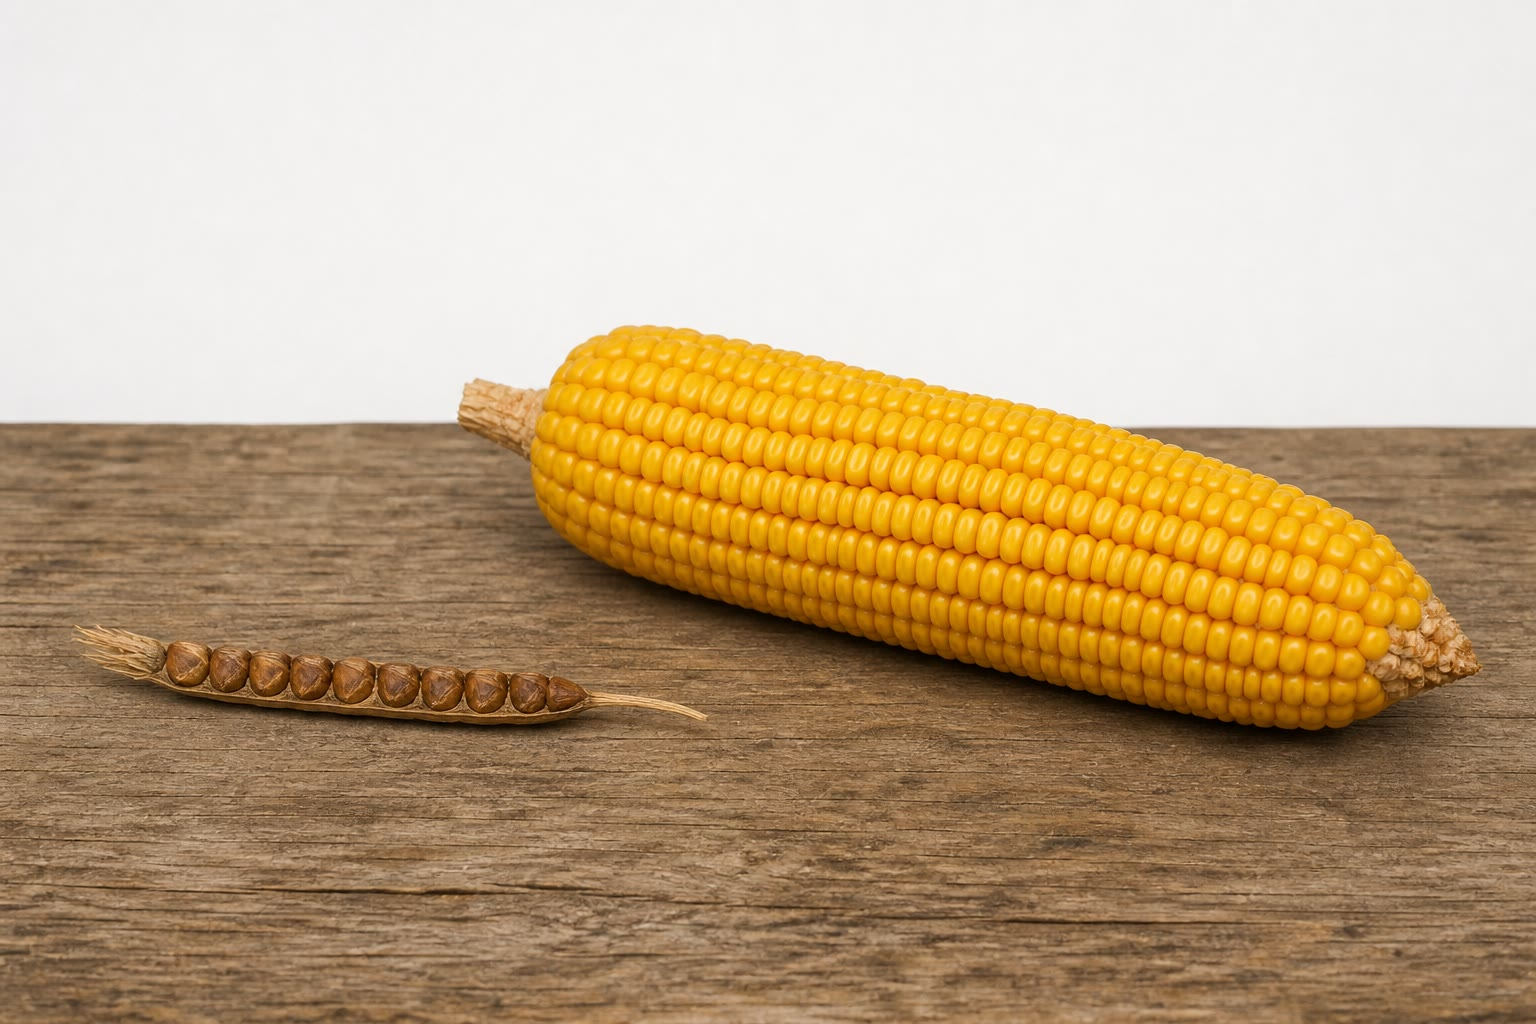
\includegraphics[width=0.62\linewidth]{images/book2/ai/g12-domestic-teosinte-maize.jpg}

{\small 大刍草与玉米。一排十二粒带壳籽粒，着生于一个脆穗上，
与之相对的是数百粒裸露籽粒，牢牢固定在穗轴上：
九千年的挑选，加上寥寥几个\omterm{def:g10:universal-dna:gene}{基因}。}
\end{omfigure}

\begin{omfigure}
\begin{tikzpicture}[font=\small, >=Stealth,
  b/.style={draw, rounded corners, align=center, text width=2.2cm, minimum height=0.9cm}]
  \node[b, fill=omMeth!15, text width=2.8cm] (wild) at (0,0) {野生甘蓝 \\ （一个物种）};
  \node[b, fill=omDef!12] (kale) at (5,3.0) {羽衣甘蓝：\\ 叶};
  \node[b, fill=omDef!12] (cab) at (5,1.8) {甘蓝：\\ 顶芽};
  \node[b, fill=omDef!12, text width=2.7cm] (spr) at (5,0.6) {球芽甘蓝：\\ 侧芽};
  \node[b, fill=omDef!12] (kohl) at (5,-0.6) {苤蓝：\\ 茎};
  \node[b, fill=omDef!12] (broc) at (5,-1.8) {西兰花：\\ 花芽};
  \node[b, fill=omDef!12] (cauli) at (5,-3.0) {花椰菜：\\ 花茎};
  \foreach \t in {kale,cab,spr,kohl,broc,cauli} \draw[->] (wild.east) -- (\t.west);
  \node[anchor=west, align=left, text width=4.6cm] at (7.2,0) {六种作物，同属一个物种：各谱系中，农民分别选择了不同器官的过度发育。六者之间仍能相互杂交。};
\end{tikzpicture}

{\small 从一个野生\omterm{def:g10:biodiversity-scales:species}{物种}经\omterm{def:g12:domesticated-plants:domestication}{人工选择}。在不同谱系中选择
叶、芽、茎或花，培育出的植株看似不同\omterm{def:g10:biodiversity-scales:species}{物种}，
实则并非如此。}
\end{omfigure}

\begin{example}[作物失去了什么]\label{ex:g12:domesticated-plants:lost}
玉米无法散播种子，栽培小麦也无法脱落籽粒；
香蕉和无籽葡萄完全不产生种子，依靠
扦插繁殖，每株都是一个克隆。作物的存续
便托付于农民，其\emph{\omterm{def:g10:biodiversity-scales:biodiversity}{遗传多样性}}随着每一阶段的选择而不断减少，
现代品种几乎完全一致，
整个地区可能只种植一个品种。野生近缘种仍然多样，
正是保存未来作物可能需要的\omterm{def:g10:universal-dna:gene}{等位基因}的地方——例如应对新病害、
适应更干燥气候的\omterm{def:g10:universal-dna:gene}{等位基因}——正是在这些地方得以保存（见\cref{ch:g10:biodiversity-scales}）。
\end{example}

\section{通过杂交育种}

\begin{proposition}[品种与杂种]\label{prop:g12:domesticated-plants:hybrids}
育种者通过杂交携带不同有利\omterm{def:g10:universal-dna:gene}{等位基因}的植株培育新品种，
并在后代中选择所需的组合，历经数代。
在玉米和许多蔬菜中，一种特殊情况占主导地位：
\emph{F1 杂种}\index{F1 杂种}。两个
自交系——各自通过数代自花授粉而变得一致且纯合——
杂交，其后代的\omterm{def:g11:enzymes-and-phenotype:phenotype}{基因型}全部相同，
在两系不同的每个\omterm{def:g10:universal-dna:gene}{基因}位点上均为杂合，并且
生长势和产量均明显高于任一亲本。再次播种时，
杂种自身的种子会发生分离，形成由生长势较弱的
植株组成的混合群体：农民每年都需购买新的杂交种子。
\end{proposition}
\admitted

\begin{omfigure}
\begin{tikzpicture}[font=\small, >=Stealth,
  b/.style={draw, rounded corners, align=center, text width=2.6cm, minimum height=1.0cm}]
  \node[b, fill=omDef!12] (a) at (0,1.2) {自交系 A\\ $AA\,bb$，一致};
  \node[b, fill=omDef!12] (bb) at (0,-1.2) {自交系 B\\ $aa\,BB$，一致};
  \node[b, fill=omMeth!20, text width=3.0cm] (f1) at (4.6,0) {F1 杂种 \\ $Aa\,Bb$，全部相同，\\ 生长旺盛};
  \node[b, fill=omProp!15, text width=3.4cm] (f2) at (9.6,0) {F2（杂种自留种子）：\\ $AA$、$Aa$、$aa$ \dots 混杂，\\ 产量降低 15--20\%};
  \draw[->] (a) -- (f1); \draw[->] (bb) -- (f1);
  \draw[->] (f1) -- node[above] {自交} (f2);
\end{tikzpicture}

{\small F1 杂种。两条纯合自交系杂交，得到整齐一致的杂合子后代，活力很强；
下一代发生分离并失去这一优势，因此种子每年都必须重新购买，
这正是种子产业的
基础。}
\end{omfigure}

\begin{omfigure}
\begin{tikzpicture}
\begin{axis}[
  width=0.86\linewidth, height=5.6cm,
  axis x line=bottom, axis y line=left,
  /pgf/number format/1000 sep={}, xmin=1900, xmax=2025, ymin=0, ymax=9,
  xlabel={年}, ylabel={小麦产量（t/ha）},
  xlabel style={font=\small, at={(axis description cs:0.5,-0.12)}, anchor=north},
  ylabel style={font=\small},
  tick label style={font=\small}, xtick={1900,1925,1950,1975,2000,2025}, ytick={0,2,4,6,8},
  clip=false,
]
\addplot[thick, omMeth, mark=*, mark size=1.5pt] coordinates
  {(1900,1.3) (1920,1.4) (1940,1.6) (1950,1.9) (1960,2.6) (1970,3.6) (1980,5.0) (1990,6.5) (2000,7.2) (2010,7.3) (2020,7.5)};
\draw[dashed, gray] (axis cs:1955,0) -- (axis cs:1955,8.5);
\node[font=\scriptsize, anchor=south, align=center] at (axis cs:1955,8.5) {矮秆品种、\\ 化肥、农药};
\end{axis}
\end{tikzpicture}

{\small 西欧某国一个世纪内的小麦平均产量（已取整）。前五十年基本持平，
此后四十年间，借助穗大、秆矮的新品种，
并辅以化肥和病虫害防治，产量增至原来的四倍。
2000 年以来的平台期
是当前育种研究的课题。}
\end{omfigure}

\begin{example}[杂种为何活力强，又为何不能持久]\label{ex:g12:domesticated-plants:vigour}
每个自交系在各位点上均为纯合，都以双拷贝携带一些弱的\omterm{def:g11:genes-and-disease:genetic}{隐性}\omterm{def:g10:universal-dna:gene}{等位基因}；
两条自交系杂交时，在两者存在差异的每个\omterm{def:g10:universal-dna:gene}{基因}位点上，
各自的弱\omterm{def:g10:universal-dna:gene}{等位基因}都被对方有功能的\omterm{def:g10:universal-dna:gene}{等位基因}掩盖。
因此 F1 为杂合子，活力强。下一代中，\omterm{def:g12:meiosis-genetic-shuffling:meiosis}{减数分裂}和受精
会再次分配\omterm{def:g10:universal-dna:gene}{等位基因}（见\cref{ch:g12:meiosis-genetic-shuffling}）：四分之一
的植株在每个\omterm{def:g10:universal-dna:gene}{基因}位点上都是弱\omterm{def:g10:universal-dna:gene}{等位基因}的纯合子，
田间因而
呈斑驳状。
\end{example}

\section{直接改变基因}

\begin{proposition}[转基因与基因编辑作物]\label{prop:g12:domesticated-plants:transgenic}
自 20 世纪 80 年代起，无需杂交即可将\omterm{def:g10:universal-dna:gene}{基因}导入植物，
即\emph{转基因技术}\index{转基因技术}（见\cref{ch:g10:universal-dna}）。
一种天然能向植物\omterm{def:g10:cells-common-unit:cell}{细胞}注入自身 \omterm{def:g10:universal-dna:information}{DNA} 片段的土壤细菌，被用作载体：
将目的\omterm{def:g10:universal-dna:gene}{基因}插入该 \omterm{def:g10:universal-dna:information}{DNA} 片段中，
再感染植物\omterm{def:g10:cells-common-unit:cell}{细胞}，并由接受该\omterm{def:g10:universal-dna:gene}{基因}的\omterm{def:g10:cells-common-unit:cell}{细胞}
再生出完整植株。目的\omterm{def:g10:universal-dna:gene}{基因}可来自任何\omterm{def:g10:biodiversity-scales:species}{物种}。
近年来，还可以在选定位置改变植物自身的\omterm{def:g10:universal-dna:gene}{基因}，
即\emph{\omterm{def:g10:universal-dna:gene}{基因}编辑}，无需引入外源 \omterm{def:g10:universal-dna:information}{DNA}。目前已获得的性状有：
对昆虫的抗性（来自细菌毒素\omterm{def:g10:universal-dna:gene}{基因}）、对除草剂的耐受性、
对病毒的抗性、水稻中的维生素前体、
成分改变的油脂。
\end{proposition}
\admitted

\begin{omfigure}
\begin{tikzpicture}[font=\small, >=Stealth,
  b/.style={draw, rounded corners, align=center, text width=2.4cm, minimum height=1.0cm}]
  \node[b, fill=omThm!12] (gene) at (0,0) {目的基因 \\ （任意物种）};
  \node[b, fill=omProp!15] (bact) at (3.3,0) {插入土壤细菌 \\ 可转移至植物的 \\ DNA 片段中};
  \node[b, fill=omDef!12] (cells) at (6.6,0) {感染植物细胞；\\ 部分细胞摄取 \\ 该基因};
  \node[b, fill=omMeth!15] (plant) at (9.9,0) {由这些细胞再生 \\ 完整植株：\\ 转基因植株};
  \draw[->] (gene) -- (bact); \draw[->] (bact) -- (cells); \draw[->] (cells) -- (plant);
\end{tikzpicture}

{\small 转\omterm{def:g10:universal-dna:gene}{基因}植物的制备。天然能将 \omterm{def:g10:universal-dna:information}{DNA} 注入植物\omterm{def:g10:cells-common-unit:cell}{细胞}的细菌，
可将所选\omterm{def:g10:universal-dna:gene}{基因}带入植物\omterm{def:g10:cells-common-unit:cell}{细胞}；
由接受该\omterm{def:g10:universal-dna:gene}{基因}的\omterm{def:g10:cells-common-unit:cell}{细胞}再生出植株，
并通过种子将其传递下去。}
\end{omfigure}

\begin{example}[玉米中的毒素基因]\label{ex:g12:domesticated-plants:bt}
一种土壤细菌能产生一种对毛毛虫有毒、而对
哺乳动物无害的\omterm{def:g11:gene-expression:protein}{蛋白质}；将其\omterm{def:g10:universal-dna:gene}{基因}导入玉米后，植株的每个\omterm{def:g10:cells-common-unit:cell}{细胞}都会产生这种毒素，
蛀食茎秆的螟虫幼虫，
咬食第一口即死亡。杀虫剂用量下降，产量
在螟虫危害严重的地区随之提高。十年之内，对该毒素产生抗性的螟虫
在连年不间断种植该作物的地区出现，这正是
\cref{ch:g11:antibiotic-resistance}中的选择在田间重演，
而如今农民被要求在转\omterm{def:g10:universal-dna:gene}{基因}玉米旁种植普通玉米作为庇护区，
以便敏感型螟虫存活，
从而稀释抗性螟虫的比例。
\end{example}

\section{取舍}

\begin{proposition}[利害所在]\label{prop:g12:domesticated-plants:stakes}
本章中的每一项技术都以新的形式提出同样的问题：
多样性的缩减（一个地区只种一个品种，
所有植株都带有同一个\omterm{def:g10:universal-dna:gene}{基因}）、农民对无法自留种子的依赖、
害虫和杂草对作物防御能力产生抗性的选择、
作物\omterm{def:g10:universal-dna:gene}{基因}借花粉扩散到野生近缘种，以及食品的安全性与所有权。
这些问题单靠生物学无法回答；
生物学所能说明的，是每项技术做了什么、没有做什么，以及它
选择了什么。
\end{proposition}
\admitted

\begin{method}[解读作物的历史]\label{met:g12:domesticated-plants:read}
\begin{enumerate}
  \item 找出野生祖先，并说明作物相对于它失去了什么
        （扩散、休眠、防御能力、多样性）。
  \item 判断这一变化是如何实现的：通过收获时的无意识选择、
        有意选择、杂交并选择、
        杂种化、\omterm{prop:g10:universal-dna:universal}{转基因技术}、\omterm{def:g10:universal-dna:gene}{基因}编辑。
  \item 统计已知涉及的\omterm{def:g10:universal-dna:gene}{基因}：\omterm{def:g12:domesticated-plants:domestication}{驯化}综合征由少数主效\omterm{def:g10:universal-dna:gene}{基因}决定，
        产量由许多微效\omterm{def:g10:universal-dna:gene}{基因}决定，
        转\omterm{def:g10:universal-dna:gene}{基因}性状则由一个\omterm{def:g10:universal-dna:gene}{基因}决定。
  \item 思考作物如今依赖什么（农民、购买的种子、
        除草剂、庇护区），以及什么又依赖于它。
\end{enumerate}
\end{method}

\begin{remark}[最古老的演化实验]\label{rem:g12:domesticated-plants:oldest}
达尔文在《\omterm{def:g10:biodiversity-scales:species}{物种}起源》一书的开篇，先谈鸽子和卷心菜，
因为育种者早已表明，选择在几个世纪内能做到什么；
他只需去掉育种者、把时间拉长。每一种作物
都是对前三章的演示：变异、选择，以及使\omterm{def:g10:biodiversity-scales:species}{物种}发生改变的频率变化，
只是以人类的速度进行，
并在每一块田地和每一个市场中留下
结果的记录。
\end{remark}

\section{练习}

\begin{exercise}[$\star$]\label{exo:g12:domesticated-plants:1}
定义\omterm{def:g12:domesticated-plants:domestication}{驯化}和\omterm{def:g12:domesticated-plants:domestication}{人工选择}。
\end{exercise}

\begin{exercise}[$\star$]\label{exo:g12:domesticated-plants:2}
列出\omterm{def:g12:domesticated-plants:domestication}{驯化}综合征的四个性状，并说明每一性状
对野生植物为何是一种不利因素。
\end{exercise}

\begin{exercise}[$\star$]\label{exo:g12:domesticated-plants:3}
什么是 F1 杂种？农民为何每年都要购买其种子？
\end{exercise}

\begin{exercise}[$\star$]\label{exo:g12:domesticated-plants:4}
如何在不经杂交的情况下将一个\omterm{def:g10:universal-dna:gene}{基因}导入植物？
\end{exercise}

\begin{exercise}[$\star$]\label{exo:g12:domesticated-plants:5}
由产量图可知，1950 年至 2000 年间，
小麦产量增长了多少倍？
\end{exercise}

\begin{exercise}[$\star\star$]\label{exo:g12:domesticated-plants:6}
解释在没有任何育种意图的情况下，用镰刀收割
如何选出了茎秆坚韧的小麦。
\end{exercise}

\begin{exercise}[$\star\star$]\label{exo:g12:domesticated-plants:7}
羽衣甘蓝、卷心菜和西兰花可以自由杂交。它们是一个\omterm{def:g10:biodiversity-scales:species}{物种}还是
三个\omterm{def:g10:biodiversity-scales:species}{物种}？是什么使它们看起来如此不同？
\end{exercise}

\begin{exercise}[$\star\star$]\label{exo:g12:domesticated-plants:8}
将两个近交系杂交。在某一\omterm{def:g10:universal-dna:gene}{基因}上，系 A 为 $AA$，
系 B 为 $aa$，求 F1 的\omterm{def:g11:enzymes-and-phenotype:phenotype}{基因型}，以及 F2 的\omterm{def:g11:enzymes-and-phenotype:phenotype}{基因型}与比例。
为何 F1 是一致的，而 F2 不一致？
\end{exercise}

\begin{exercise}[$\star\star$]\label{exo:g12:domesticated-plants:9}
为何在产毒玉米的田间会出现抗性螟虫，
以及普通玉米构成的庇护区如何减缓它们的发展？
\end{exercise}

\begin{exercise}[$\star\star$]\label{exo:g12:domesticated-plants:10}
大刍草与玉米在约五个主效\omterm{def:g10:universal-dna:gene}{基因}上存在差异。请解释为何如此少的
\omterm{def:g10:universal-dna:gene}{基因}能使植物发生如此大的变化，并利用
\cref{ch:g12:diversification-of-life}加以说明。
\end{exercise}

\begin{exercise}[$\star\star$]\label{exo:g12:domesticated-plants:11}
为何要将作物的野生近缘种保存在种子库中，
尽管它们几乎没有产量？
\end{exercise}

\begin{exercise}[$\star\star\star$]\label{exo:g12:domesticated-plants:12}
将一种耐除草剂油菜种植在一种可与之杂交的野芥菜旁边。
预测若干年后可能发生的情况，
并指出涉及的前几章中的相关过程。
\end{exercise}

\begin{exercise}[$\star\star\star$]\label{exo:g12:domesticated-plants:13}
自 2000 年以来，产量曲线已趋于平坦。提出两个生物学原因
和一个非生物学原因，并说明育种者可以尝试什么。
\end{exercise}

\begin{exercise}[$\star\star\star$]\label{exo:g12:domesticated-plants:14}
从三个方面比较通过杂交与选择获得的品种，
以及通过转\omterm{def:g10:universal-dna:gene}{基因}获得的品种：
新\omterm{def:g10:universal-dna:gene}{等位基因}的来源、改变的\omterm{def:g10:universal-dna:gene}{基因}数目以及所需时间。
\end{exercise}

\begin{exercise}[$\star\star\star$]\label{exo:g12:domesticated-plants:15}
“\omterm{def:g12:domesticated-plants:domestication}{驯化}是\omterm{def:g12:selection-drift-speciation:selection}{自然选择}的反面。”请写一段话讨论，
结合\omterm{def:g12:selection-drift-speciation:population}{等位基因频率}的计算、选择的动因，
以及被选择植物的命运。
\end{exercise}

\section{问题：九千年，五个基因}

\begin{problem}[{周末问题——由大刍草培育玉米：
比较穗子，计算选择，追踪 F2 中杂种的产量，
并管理针对抗性的毒素基因}]
\label{pb:g12:domesticated-plants:1}
一株大刍草的穗轴上着生 12 粒种子，每粒 \qty{0.08}{g}，外有坚硬的壳，
穗轴易碎；一个玉米果穗上有 600 粒种子，
每粒 \qty{0.3}{g}，裸露，着生于坚硬的穗轴上。玉米约在 9000
年前被\omterm{def:g12:domesticated-plants:domestication}{驯化}；一代即一年。

\medskip
\noindent\textbf{第一部分——穗子。}
\begin{enumerate}
  \item 计算大刍草和玉米每个穗子中种子的质量，
        以及二者之间的倍数关系。
  \item 列出玉米果穗中属于
        \omterm{def:g12:domesticated-plants:domestication}{驯化}综合征的性状，并对每一个性状说明
        其对野生植物为何是不利的。
  \item 有壳种子由一个\omterm{def:g10:universal-dna:gene}{基因}控制，裸露\omterm{def:g10:universal-dna:gene}{等位基因}
        为\omterm{def:g11:genes-and-disease:genetic}{隐性}。解释为何最早的农民只能在田间
        发现少数裸露种子的植株，它们是
        罕见个体。
  \item 假设裸露\omterm{def:g10:universal-dna:gene}{等位基因}在野生\omterm{def:g12:selection-drift-speciation:population}{种群}中的频率为 0.01，
        求表现为裸露种子的植株所占的比例。
  \item 一位农民只播种裸露种子植株的种子。
        求其下一代作物中裸露\omterm{def:g10:universal-dna:gene}{等位基因}的频率。
\end{enumerate}

\medskip
\noindent\textbf{第二部分——九千代。}
\begin{enumerate}[resume]
  \item 穗上的籽粒数在 9000 代中由 12 增至 600。
        计算每代的平均增长倍数。
        为何每代如此微小的变化已足以造成这样的改变？
  \item 穗行数受许多微效\omterm{def:g10:universal-dna:gene}{基因}控制。
        试解释为何这样的性状会在选择作用下逐步、长期地响应，
        而有壳籽粒性状
        却在一步之内发生改变。
  \item 玉米仍能与大刍草杂交并产生可育后代。
        它们是否属于同一\omterm{def:g10:biodiversity-scales:species}{物种}？
        \omterm{def:g12:domesticated-plants:domestication}{驯化}改变了哪些方面，又未改变哪些方面？
  \item 现代品种在遗传上是一致的。
        指出由此产生的风险，以及用来应对该风险的资源。
  \item 玉米无法扩散其种子。
        就选择作用而言，这一点说明了植物与农民
        之间的关系意味着什么？
\end{enumerate}

\medskip
\noindent\textbf{第三部分——杂种。}
自交系 A 的产量为 \qty{5}{t/ha}，B 系为 \qty{5.5}{t/ha}，其 \omterm{prop:g12:domesticated-plants:hybrids}{F1
杂种}为 \qty{10}{t/ha}；由该杂种种子长成的 F2 产量为
\qty{8.2}{t/ha}。杂种种子的成本相当于 \qty{0.4}{t/ha}
的玉米。
\begin{enumerate}[resume]
  \item F1 比较优亲本高出百分之几？
        F2 比 F1 低百分之几？
  \item 利用\cref{ex:g12:domesticated-plants:vigour}中的\omterm{def:g11:enzymes-and-phenotype:phenotype}{基因型}，
        解释 F1 的杂种优势以及 F2 的衰退。
  \item 一位农民在每年购买杂交种子与留用 F1 种子之间犹豫不决。
        比较两种做法的净收获，
        并说明种子公司的业务为何存在。
  \item 为何不能直接把自交系卖给农民，
        让他们自行配制杂种？
  \item 杂种体系对田间的\omterm{def:g10:biodiversity-scales:biodiversity}{遗传多样性}产生了什么影响，
        对农民的独立性又产生了什么影响？
\end{enumerate}

\medskip
\noindent\textbf{第四部分——毒素\omterm{def:g10:universal-dna:gene}{基因}。}
一个螟虫\omterm{def:g12:selection-drift-speciation:population}{种群}中，抗性\omterm{def:g10:universal-dna:gene}{等位基因}的频率为 0.001，
该抗性\omterm{def:g10:universal-dna:gene}{等位基因}为\omterm{def:g11:genes-and-disease:genetic}{隐性}；仅 $rr$ \omterm{def:g11:enzymes-and-phenotype:phenotype}{基因型}的螟虫能在毒素玉米上存活。
\begin{enumerate}[resume]
  \item 第一年，在毒素玉米田中存活的螟虫占多大比例？
        计算存活个体中
        $r$ 的频率。
  \item 试解释：在没有庇护所的情况下，抗性为何会在几年内扩散，
        以\omterm{def:g11:antibiotic-resistance:antibiotic}{抗生素}为模型加以说明。
  \item 一块普通玉米构成的庇护所，使毒素田旁边保有大量
        敏感螟虫。试解释这如何使抗性\omterm{def:g10:universal-dna:gene}{等位基因}保持稀少，
        并利用抗性存活个体与庇护所螟虫
        所产后代的\omterm{def:g11:enzymes-and-phenotype:phenotype}{基因型}加以说明。
  \item 比较庇护所与\omterm{def:g11:antibiotic-resistance:antibiotic}{抗生素}的“完整疗程”，
        两者有何相同，又有何不同？
  \item 陈述结论：\omterm{def:g12:domesticated-plants:domestication}{驯化}使穗上籽粒数增加的倍数，
        所需主要\omterm{def:g10:universal-dna:gene}{基因}的数目，
        以及它所造成的唯一依赖关系。
\end{enumerate}
\end{problem}
